\documentclass[11pt,a4paper]{report}
\usepackage[textwidth=37em,vmargin=30mm]{geometry}
\usepackage{calc,xunicode,amsmath,amssymb,paralist,enumitem,tabu,booktabs,datetime2,xeCJK,xeCJKfntef,listings}
\usepackage{tocloft,fancyhdr,tcolorbox,xcolor,graphicx,eso-pic,xltxtra,xelatexemoji}

\newcommand{\envyear}[0]{2025}
\newcommand{\envdatestr}[0]{2025-01-12}
\newcommand{\envfinaldir}[0]{webdb/2025/20250112/final}

\usepackage[hidelinks]{hyperref}
\hypersetup{
    colorlinks=false,
    pdfpagemode=FullScreen,
    pdftitle={Web Digest - \envdatestr}
}

\setlength{\cftbeforechapskip}{10pt}
\renewcommand{\cftchapfont}{\rmfamily\bfseries\large\raggedright}
\setlength{\cftbeforesecskip}{2pt}
\renewcommand{\cftsecfont}{\sffamily\small\raggedright}

\setdefaultleftmargin{2em}{2em}{1em}{1em}{1em}{1em}

\usepackage{xeCJK,xeCJKfntef}
\xeCJKsetup{PunctStyle=plain,RubberPunctSkip=false,CJKglue=\strut\hskip 0pt plus 0.1em minus 0.05em,CJKecglue=\strut\hskip 0.22em plus 0.2em}
\XeTeXlinebreaklocale "zh"
\XeTeXlinebreakskip = 0pt


\setmainfont{Brygada 1918}
\setromanfont{Brygada 1918}
\setsansfont{IBM Plex Sans}
\setmonofont{JetBrains Mono NL}
\setCJKmainfont{Noto Serif CJK SC}
\setCJKromanfont{Noto Serif CJK SC}
\setCJKsansfont{Noto Sans CJK SC}
\setCJKmonofont{Noto Sans CJK SC}

\setlength{\parindent}{0pt}
\setlength{\parskip}{8pt}
\linespread{1.15}

\lstset{
	basicstyle=\ttfamily\footnotesize,
	numbersep=5pt,
	backgroundcolor=\color{black!5},
	showspaces=false,
	showstringspaces=false,
	showtabs=false,
	tabsize=2,
	captionpos=b,
	breaklines=true,
	breakatwhitespace=true,
	breakautoindent=true,
	linewidth=\textwidth
}






\newcommand{\coverpic}[2]{
    % argv: itemurl, authorname
    Cover photo by #2~~(\href{#1}{#1})
}
\newcommand{\makeheader}[0]{
    \begin{titlepage}
        % \newgeometry{hmargin=15mm,tmargin=21mm,bmargin=12mm}
        \begin{center}
            
            \rmfamily\scshape
            \fontspec{BaskervilleF}
            \fontspec{Old Standard}
            \fontsize{59pt}{70pt}\selectfont
            WEB\hfill DIGEST
            
            \vfill
            % \vskip 30pt
            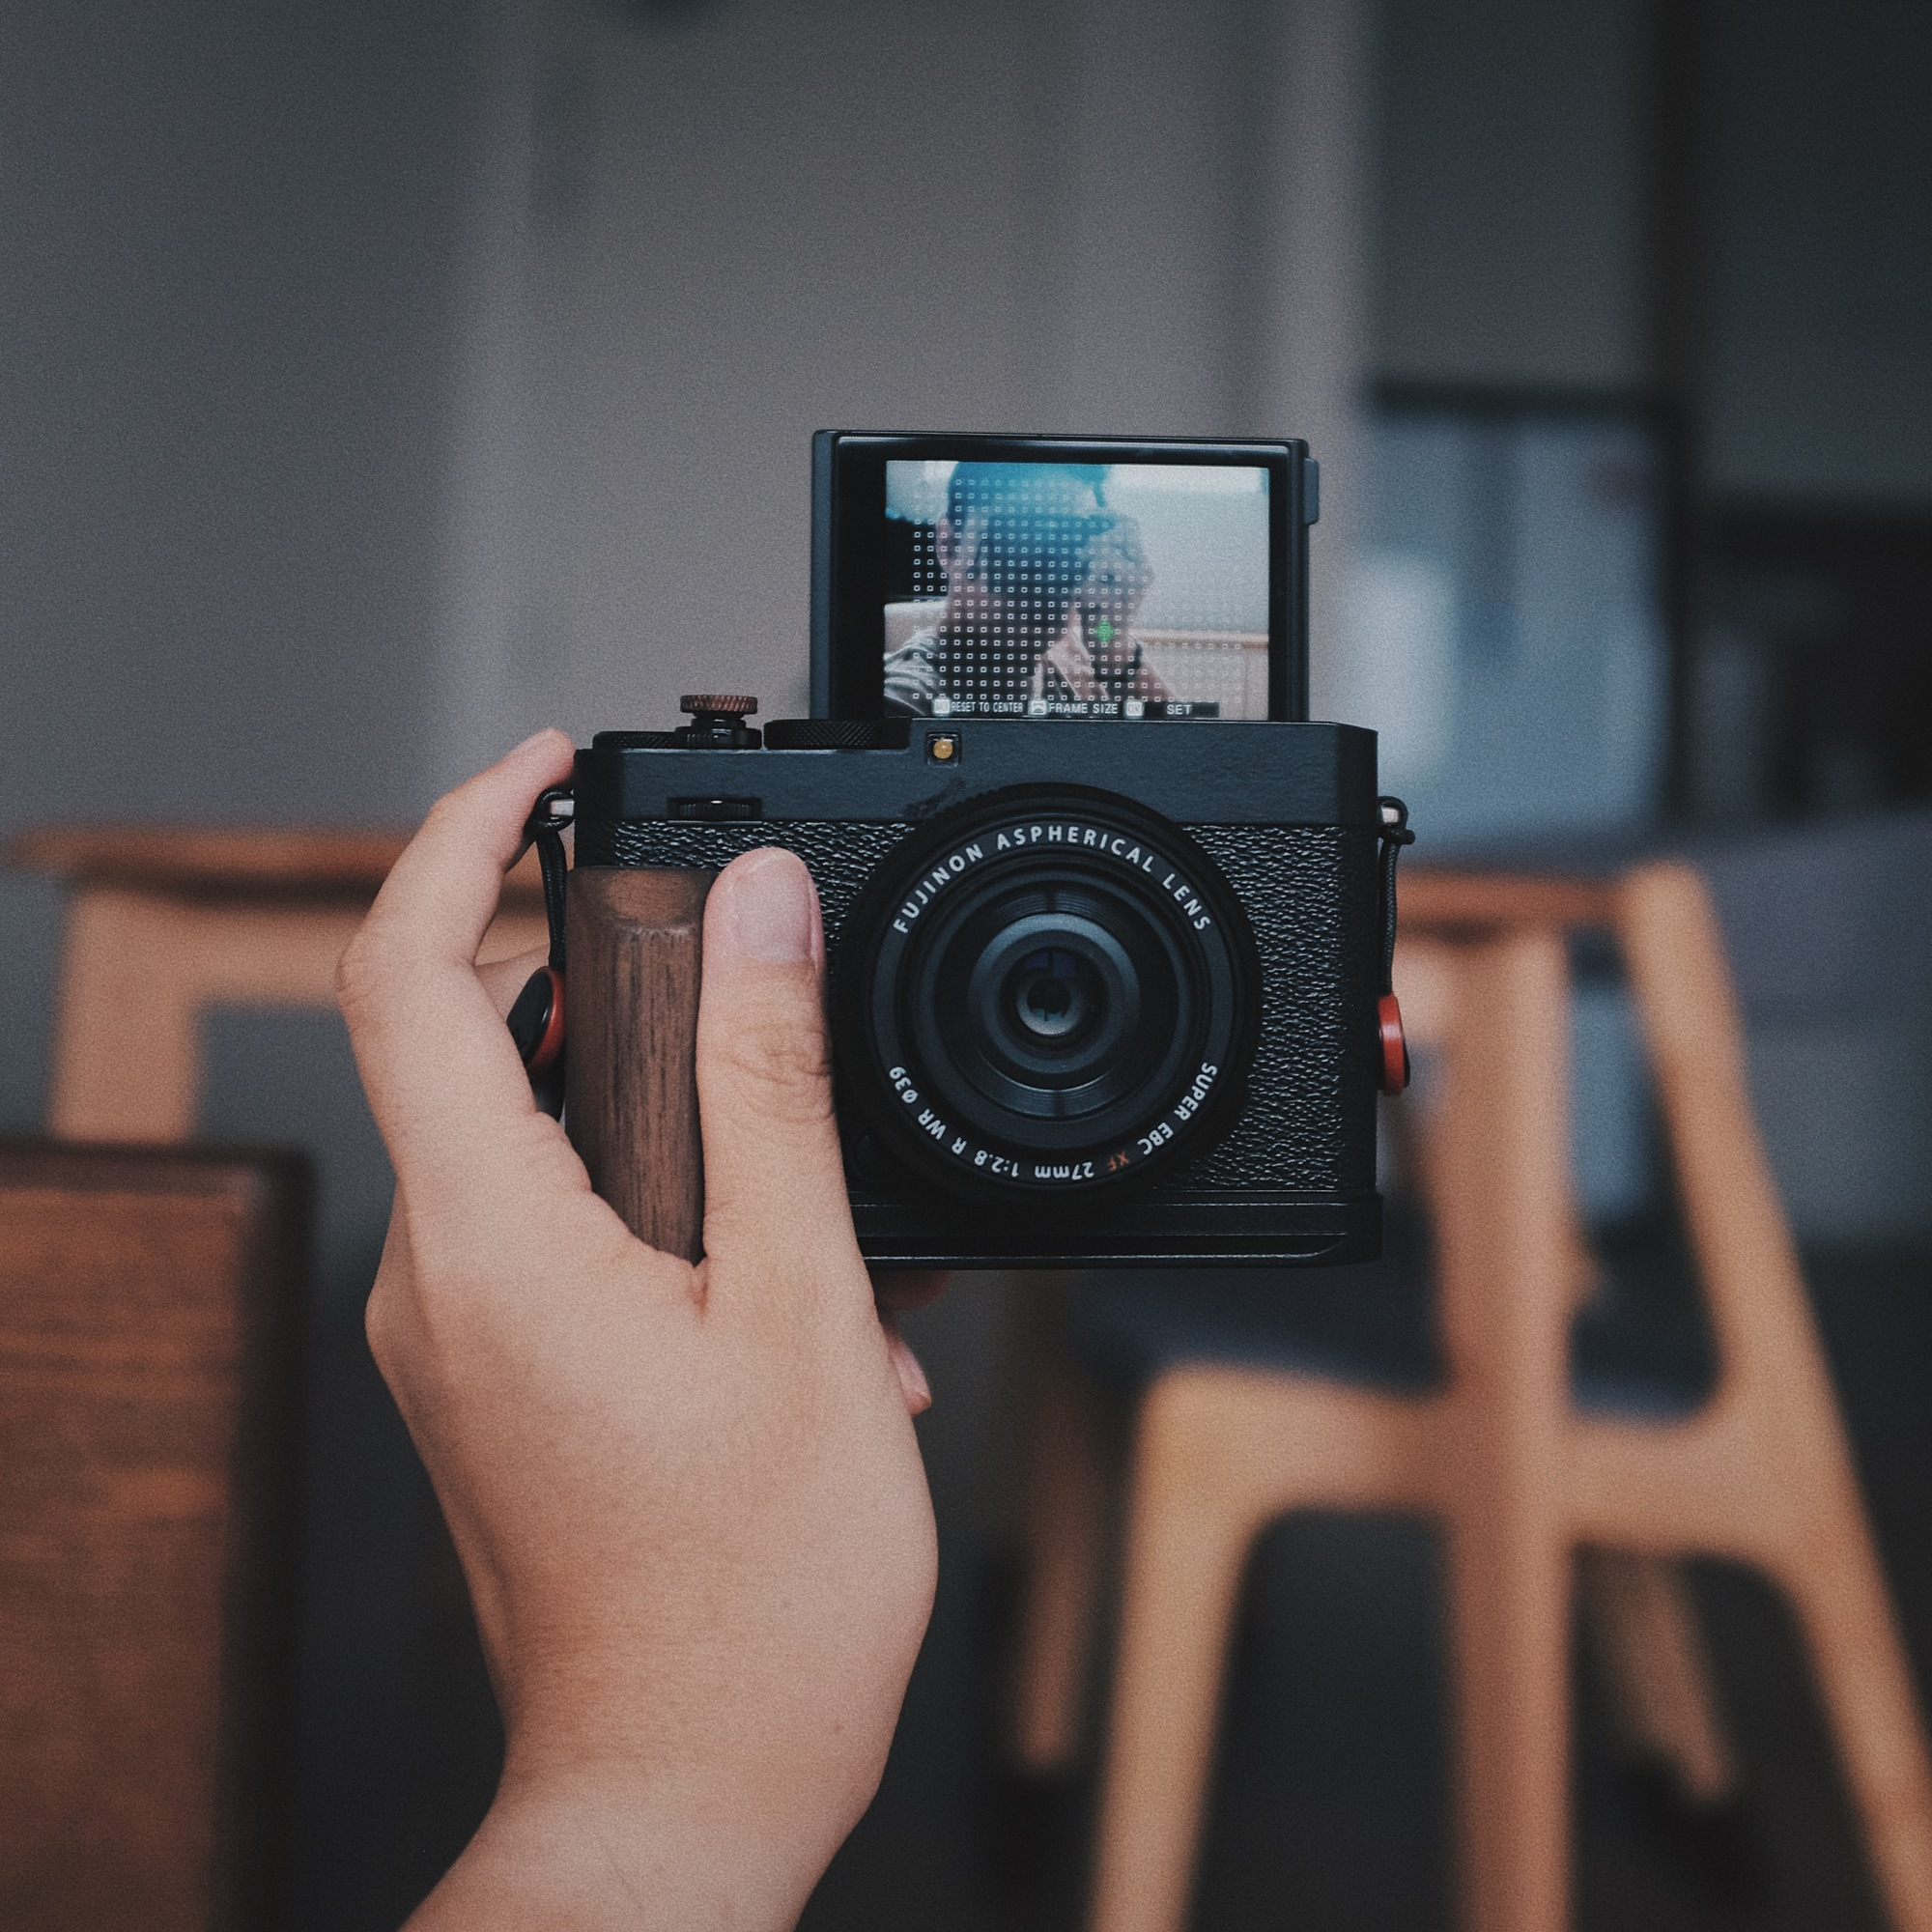
\includegraphics[width=\linewidth]{\envfinaldir/coverpic-prod.jpg}\par
            % \vskip 30pt
            \vfill

            \normalsize\rmfamily\scshape
            \copyright{} The Web Digest Project \hfill\large \envdatestr
        \end{center}
    \end{titlepage}
    % \restoregeometry
}
\newcommand{\simplehref}[1]{%
    \textcolor{blue!80!green}{\href{#1}{#1}}%
}
\renewcommand{\contentsname}{\center\Huge\sffamily\bfseries Contents\par\vskip 20pt}
\newcounter{ipartcounter}
\setcounter{ipartcounter}{0}
\newcommand{\ipart}[1]{
    % \vskip 20pt
    \clearpage
    \stepcounter{ipartcounter}
    \phantomsection
    \addcontentsline{toc}{chapter}{#1}
    % \begin{center}
    %     \Huge
    %     \sffamily\bfseries
    %     #1
    % \end{center}
    % \vskip 20pt plus 7pt
}
\newcounter{ichaptercounter}
\setcounter{ichaptercounter}{0}
\newcommand{\ichapter}[1]{
    % \vskip 20pt
    \clearpage
    \stepcounter{ichaptercounter}
    \phantomsection
    \addcontentsline{toc}{section}{\numberline{\arabic{ichaptercounter}}#1}
    \begin{center}
        \Huge
        \sffamily\bfseries
        #1
    \end{center}
    \vskip 20pt plus 7pt
}
\newcommand{\entrytitlefont}[1]{\subsection*{\raggedright\Large\sffamily\bfseries#1}}
\newcommand{\entryitemGeneric}[2]{
    % argv: title, url
    \parbox{\linewidth}{
        \entrytitlefont{#1}\par\vskip 5pt
        \footnotesize\ttfamily\mdseries
        \simplehref{#2}
    }\vskip 11pt plus 11pt minus 1pt
}
\newcommand{\entryitemGithub}[3]{
    % argv: title, url, desc
    \parbox{\linewidth}{
        \entrytitlefont{#1}\par\vskip 5pt
        \footnotesize\ttfamily\mdseries
        \simplehref{#2}\par\vskip 5pt
        \small\rmfamily\mdseries#3
    }\vskip 11pt plus 11pt minus 1pt
}
\newcommand{\entryitemAp}[3]{
    % argv: title, url, desc
    \parbox{\linewidth}{
        \entrytitlefont{#1}\par\vskip 5pt
        \footnotesize\ttfamily\mdseries
        \simplehref{#2}\par\vskip 5pt
        \small\rmfamily\mdseries#3
    }\vskip 11pt plus 11pt minus 1pt
}
\newcommand{\entryitemHackernews}[3]{
    % argv: title, hnurl, rawurl
    % \parbox{\linewidth}{
    %     \entrytitlefont{#1}\par\vskip 5pt
    %     \footnotesize\ttfamily\mdseries
    %     \simplehref{#3}\par
    %     \textcolor{black!50}{\href{#2}{#2}}
    % }\vskip 11pt plus 11pt minus 1pt
    \begin{minipage}{\linewidth}
            \entrytitlefont{#1}\par\vskip 5pt
            \footnotesize\ttfamily\mdseries
            \simplehref{#3}\par
            \textcolor{black!50}{\href{#2}{#2}}
    \end{minipage}\par\vskip 11pt plus 11pt minus 1pt
}







\begin{document}

\makeheader

\tableofcontents\clearpage




\ipart{Developers}
\ichapter{Hacker News}
\entryitemTwoLinks{Matt Mullenweg deactivates WordPress accounts of contributors planning a fork}{https://news.ycombinator.com/item?id=42667766}{https://techcrunch.com/2025/01/11/matt-mullenweg-deactivates-wordpress-accounts-of-contributors-planning-a-fork/}

\entryitemTwoLinks{De-smarting the Marshall Uxbridge Bluetooth speaker}{https://news.ycombinator.com/item?id=42666572}{https://tomscii.sig7.se/2025/01/De-smarting-the-Marshall-Uxbridge}

\entryitemTwoLinks{Show HN: TypeScript/React/Vue Window Layout Manager (Tabs, Floating, Popouts)}{https://news.ycombinator.com/item?id=42666492}{https://github.com/mathuo/dockview}

\entryitemTwoLinks{Show HN: A Better Log Service}{https://news.ycombinator.com/item?id=42666139}{https://txtlog.net/}

\entryitemTwoLinks{Track your devices via Apple FindMy network in Go/TinyGo}{https://news.ycombinator.com/item?id=42665367}{https://github.com/hybridgroup/go-haystack}

\entryitemTwoLinks{The State of Vim}{https://news.ycombinator.com/item?id=42665222}{https://lwn.net/SubscriberLink/1002342/a8d8a17f30968b93/}

\entryitemTwoLinks{Ingrid Daubechies Awarded National Medal of Science}{https://news.ycombinator.com/item?id=42664893}{https://today.duke.edu/2025/01/ingrid-daubechies-awarded-national-medal-science}

\entryitemTwoLinks{PrivTracker – Private BitTorrent tracker for everyone}{https://news.ycombinator.com/item?id=42664409}{https://privtracker.com/}

\entryitemTwoLinks{Nearly all binary searches and mergesorts are broken (2006)}{https://news.ycombinator.com/item?id=42664400}{https://research.google/blog/extra-extra-read-all-about-it-nearly-all-binary-searches-and-mergesorts-are-broken/}

\entryitemTwoLinks{Be Aware of the Makefile Effect}{https://news.ycombinator.com/item?id=42663231}{https://blog.yossarian.net/2025/01/10/Be-aware-of-the-Makefile-effect}

\entryitemTwoLinks{The Anti-Social Century}{https://news.ycombinator.com/item?id=42662340}{https://www.theatlantic.com/magazine/archive/2025/02/american-loneliness-personality-politics/681091/}

\entryitemTwoLinks{Very Wrong Math}{https://news.ycombinator.com/item?id=42661432}{https://www.charlespetzold.com/blog/2025/01/Very-Wrong-Math.html}

\entryitemTwoLinks{Portals and Quake}{https://news.ycombinator.com/item?id=42661185}{https://30fps.net/pages/pvs-portals-and-quake/}

\entryitemTwoLinks{Building Bauble}{https://news.ycombinator.com/item?id=42660942}{https://ianthehenry.com/posts/bauble/building-bauble/}

\entryitemTwoLinks{Cannonball: An Enhanced OutRun Engine}{https://news.ycombinator.com/item?id=42660848}{https://github.com/djyt/cannonball}

\entryitemTwoLinks{OpenAI's bot crushed this seven-person company's web site 'like a DDoS attack'}{https://news.ycombinator.com/item?id=42660377}{https://techcrunch.com/2025/01/10/how-openais-bot-crushed-this-seven-person-companys-web-site-like-a-ddos-attack/}

\entryitemTwoLinks{Phi-4 Bug Fixes}{https://news.ycombinator.com/item?id=42660335}{https://unsloth.ai/blog/phi4}

\entryitemTwoLinks{Flattening ASTs and other compiler data structures (2023)}{https://news.ycombinator.com/item?id=42659061}{https://www.cs.cornell.edu/~asampson/blog/flattening.html}

\entryitemTwoLinks{Cuttle – a MTG like game using a standard 52 card deck}{https://news.ycombinator.com/item?id=42658614}{https://www.pagat.com/combat/cuttle.html}

\entryitemTwoLinks{Meta's memo to employees rolling back DEI programs}{https://news.ycombinator.com/item?id=42657901}{https://www.axios.com/2025/01/10/meta-dei-memo-employees-programs}\ichapter{Phoronix}
\entryitemGeneric{\hskip 0pt{}Fedora 42 Looks To Ship Optimized Executables For Different x86\_64 Capabilities}{https://www.phoronix.com/news/Fedora-42-Optimized-Executables}

\entryitemGeneric{\hskip 0pt{}Debian 12.9 Released With Various Security \& Bug Fixes}{https://www.phoronix.com/news/Debian-12.9-Released}

\entryitemGeneric{\hskip 0pt{}AMD Preps More GPU Driver Fixes For Linux 6.14, Cleaner Shader For RDNA2 dGPUs}{https://www.phoronix.com/news/Linux-6.14-Cleaner-Shader-RDNA2}

\entryitemGeneric{\hskip 0pt{}Intel Xe Driver Adding "RPa" Frequency Reporting With Linux 6.14}{https://www.phoronix.com/news/Intel-Xe-Driver-RPa-Frequency}

\entryitemGeneric{\hskip 0pt{}GNOME Image Viewer Now Editing JPEGs, Other GNOME 48 Progress}{https://www.phoronix.com/news/GNOME-48-Editing-JPEGs}

\entryitemGeneric{\hskip 0pt{}Sony Proposes Changing LLVM Clang Default To C++20 Mode}{https://www.phoronix.com/news/Sony-LLVM-Clang-CXX20-Default}

\entryitemGeneric{\hskip 0pt{}KDE Plasma 6.3 Bringing A More Consistent Close Button, Other Last Minute Changes}{https://www.phoronix.com/news/KDE-Plasma-6.3-Close-Button}

\entryitemGeneric{\hskip 0pt{}Intel Open-Source Vulkan Driver Merges Initial AV1 Decode Support}{https://www.phoronix.com/news/Intel-Vulkan-Video-AV1-Decode}

\entryitemGeneric{\hskip 0pt{}Wine 10.0-rc5 Brings Another 31 Bug Fixes}{https://www.phoronix.com/news/Wine-10.0-rc5}\ichapter{Dribbble}
\entryitemGeneric{\hskip 0pt{}Cub Studio Process}{https://dribbble.com/shots/25456521-Cub-Studio-Process}

\entryitemGeneric{\hskip 0pt{}Polar Bear + Baby (2012)}{https://dribbble.com/shots/25454483-Polar-Bear-Baby-2012}

\entryitemGeneric{\hskip 0pt{}SHOWREEL 24'}{https://dribbble.com/shots/25450148-SHOWREEL-24}

\entryitemGeneric{\hskip 0pt{}Southland Provisions}{https://dribbble.com/shots/25456279-Southland-Provisions}

\entryitemGeneric{\hskip 0pt{}Cromatic.bio®}{https://dribbble.com/shots/25451539-Cromatic-bio}

\entryitemGeneric{\hskip 0pt{}Business set}{https://dribbble.com/shots/25444987-Business-set}

\entryitemGeneric{\hskip 0pt{}Running Dog Logo}{https://dribbble.com/shots/25450403-Running-Dog-Logo}

\entryitemGeneric{\hskip 0pt{}Pageless Logo \& Visual Identity}{https://dribbble.com/shots/25450527-Pageless-Logo-Visual-Identity}

\entryitemGeneric{\hskip 0pt{}B}{https://dribbble.com/shots/25449124-B}

\entryitemGeneric{\hskip 0pt{}Tempest Logo Design \& Visual Identity}{https://dribbble.com/shots/25371917-Tempest-Logo-Design-Visual-Identity}

\entryitemGeneric{\hskip 0pt{}HR Management Dashboard}{https://dribbble.com/shots/25442919-HR-Management-Dashboard}

\entryitemGeneric{\hskip 0pt{}Milky Giant Studios Logo}{https://dribbble.com/shots/25403425-Milky-Giant-Studios-Logo}

\entryitemGeneric{\hskip 0pt{}Cute Chicken Logo}{https://dribbble.com/shots/25443854-Cute-Chicken-Logo}

\entryitemGeneric{\hskip 0pt{}Bexet}{https://dribbble.com/shots/25440591-Bexet}

\entryitemGeneric{\hskip 0pt{}Down the drain}{https://dribbble.com/shots/25445263-Down-the-drain}

\entryitemGeneric{\hskip 0pt{}Placefully - Logo Design}{https://dribbble.com/shots/25437901-Placefully-Logo-Design}

\entryitemGeneric{\hskip 0pt{}Portex}{https://dribbble.com/shots/25434801-Portex}

\entryitemGeneric{\hskip 0pt{}Vox - Brandmark}{https://dribbble.com/shots/25429765-Vox-Brandmark}

\entryitemGeneric{\hskip 0pt{}Dropbox - Logo Redesign}{https://dribbble.com/shots/25432726-Dropbox-Logo-Redesign}

\entryitemGeneric{\hskip 0pt{}Logo Design 2 for Ai Assistant (Unused for Sale)}{https://dribbble.com/shots/25433244-Logo-Design-2-for-Ai-Assistant-Unused-for-Sale}

\entryitemGeneric{\hskip 0pt{}Run it back}{https://dribbble.com/shots/25430165-Run-it-back}

\entryitemGeneric{\hskip 0pt{}Behemoths}{https://dribbble.com/shots/25433176-Behemoths}

\entryitemGeneric{\hskip 0pt{}Alder Posters}{https://dribbble.com/shots/25433543-Alder-Posters}

\entryitemGeneric{\hskip 0pt{}Hooke Outdoor Co.}{https://dribbble.com/shots/25429227-Hooke-Outdoor-Co}


\ipart{Developers~~~~(zh-Hans)}
\ichapter{Solidot}
\entryitemGeneric{\hskip 0pt{}物理学家发现新粒子分数激子}{https://www.solidot.org/story?sid=80307}

\entryitemGeneric{\hskip 0pt{}YouTube 主播向 AI 公司出售未发布视频去训练 AI}{https://www.solidot.org/story?sid=80306}

\entryitemGeneric{\hskip 0pt{}世界最强超算 El Capitan 正式启用}{https://www.solidot.org/story?sid=80305}

\entryitemGeneric{\hskip 0pt{}StackOverflow 新问题数量大幅减少}{https://www.solidot.org/story?sid=80304}

\entryitemGeneric{\hskip 0pt{}德国众多大学机构集体宣布退出 X}{https://www.solidot.org/story?sid=80303}

\entryitemGeneric{\hskip 0pt{}Automattic 大幅缩减对 WordPress.org 的支持}{https://www.solidot.org/story?sid=80302}

\entryitemGeneric{\hskip 0pt{}巴西给 Meta 72 小时时间解释其事实核查政策的变化}{https://www.solidot.org/story?sid=80301}

\entryitemGeneric{\hskip 0pt{}独立分析认为巴勒斯坦卫生部严重低估了加沙死亡人数}{https://www.solidot.org/story?sid=80300}

\entryitemGeneric{\hskip 0pt{}四分之一淡水动物面临灭绝}{https://www.solidot.org/story?sid=80299}

\entryitemGeneric{\hskip 0pt{}美国司法部准备出售扣押的丝绸之路比特币}{https://www.solidot.org/story?sid=80298}

\entryitemGeneric{\hskip 0pt{}法官拒绝了试图从垃圾堆里挖出 8000 比特币的诉讼}{https://www.solidot.org/story?sid=80297}

\entryitemGeneric{\hskip 0pt{}三星量产笔记本用的卷轴 OLED 显示屏}{https://www.solidot.org/story?sid=80296}

\entryitemGeneric{\hskip 0pt{}2024 年是平均气温比工业化前水平高出1.5 摄氏度的第一年}{https://www.solidot.org/story?sid=80295}

\entryitemGeneric{\hskip 0pt{}氟化物暴露与 IQ 分数低相关}{https://www.solidot.org/story?sid=80294}

\entryitemGeneric{\hskip 0pt{}中国在前沿 AI 研究上紧追美国}{https://www.solidot.org/story?sid=80293}

\entryitemGeneric{\hskip 0pt{}中国风投让失败的创业者成为失信债务人}{https://www.solidot.org/story?sid=80292}

\entryitemGeneric{\hskip 0pt{}ispace 准备再次发射登月舱}{https://www.solidot.org/story?sid=80291}

\entryitemGeneric{\hskip 0pt{}乳腺癌是最常见的癌症肺癌是最致命的癌症}{https://www.solidot.org/story?sid=80290}

\entryitemGeneric{\hskip 0pt{}拜登计划在离任前对 AI 芯片出口实施新限制}{https://www.solidot.org/story?sid=80289}

\entryitemGeneric{\hskip 0pt{}VLC 预览本地 AI 字幕翻译功能}{https://www.solidot.org/story?sid=80288}\ichapter{V2EX}
\entryitemGeneric{\hskip 0pt{}[程序员] 关于不想读代码}{https://www.v2ex.com/t/1104442}

\entryitemGeneric{\hskip 0pt{}[FFmpeg] FFmpegKit has been officially retired. There will be no further ffmpeg-kit releases.}{https://www.v2ex.com/t/1104441}

\entryitemGeneric{\hskip 0pt{}[问与答] 之前买的教育邮箱用了一年 jetbrain 全家桶}{https://www.v2ex.com/t/1104440}

\entryitemGeneric{\hskip 0pt{}[宽带症候群] 芬兰赫尔辛基已更新 2.5G 对等宽带}{https://www.v2ex.com/t/1104438}

\entryitemGeneric{\hskip 0pt{}[生活] 想看看大家的桌面环境}{https://www.v2ex.com/t/1104436}

\entryitemGeneric{\hskip 0pt{}[全球工单系统] Firefox 浏览器的 http/3 是不是有 bug ?}{https://www.v2ex.com/t/1104435}

\entryitemGeneric{\hskip 0pt{}[分享创造] 用 GPT 写了一个前台窗口检测工具}{https://www.v2ex.com/t/1104434}

\entryitemGeneric{\hskip 0pt{}[生活] 婚姻就是男人的坟墓,而我,已是那将死之人}{https://www.v2ex.com/t/1104431}

\entryitemGeneric{\hskip 0pt{}[职场话题] 非统本该何去何从}{https://www.v2ex.com/t/1104430}

\entryitemGeneric{\hskip 0pt{}[硬件] espidf 上面 ble mesh 的开发中,如何给节点的多个 element 绑定密钥?}{https://www.v2ex.com/t/1104429}

\entryitemGeneric{\hskip 0pt{}[分享发现] tg 空投 duckchain, 1/16 上市}{https://www.v2ex.com/t/1104428}

\entryitemGeneric{\hskip 0pt{}[酷工作] [北京/上海/深圳] Meshy 招全职后端 / 前端 不加班不打卡}{https://www.v2ex.com/t/1104427}

\entryitemGeneric{\hskip 0pt{}[Android] 2025 年 1 月帮推荐个安卓手机}{https://www.v2ex.com/t/1104426}

\entryitemGeneric{\hskip 0pt{}[分享发现] 无人机低空经济落地}{https://www.v2ex.com/t/1104425}

\entryitemGeneric{\hskip 0pt{}[分享发现] 推荐一个可以把 B 站频道转成视频播客的开源项目 podcast2}{https://www.v2ex.com/t/1104424}

\entryitemGeneric{\hskip 0pt{}[Apple] 今天一时兴起买了个 iPad air 体验不是很好}{https://www.v2ex.com/t/1104423}

\entryitemGeneric{\hskip 0pt{}[奇思妙想] 产品构想: 脖饰电极 (AI 眼镜辅助续航)}{https://www.v2ex.com/t/1104422}

\entryitemGeneric{\hskip 0pt{}[问与答] 请问广东联通 iptv 盒子连接联通 cpe 可以看电视直播吗?}{https://www.v2ex.com/t/1104421}

\entryitemGeneric{\hskip 0pt{}[硬件] 亮机卡还可能和主板不兼容吗?}{https://www.v2ex.com/t/1104420}

\entryitemGeneric{\hskip 0pt{}[随想] 平价洗衣店}{https://www.v2ex.com/t/1104419}

\entryitemGeneric{\hskip 0pt{}[程序员] 我也来问 12306 的库存方面的问题}{https://www.v2ex.com/t/1104418}

\entryitemGeneric{\hskip 0pt{}[Apple] 有望推动 Apple 智能落地中国:苹果成立上海新公司,注册资本 3500 万美元}{https://www.v2ex.com/t/1104417}

\entryitemGeneric{\hskip 0pt{}[投资] 冷门问题:有美股投资者参与过针对公司的集体诉讼索赔吗,不知道非美国人容不容易参与}{https://www.v2ex.com/t/1104414}

\entryitemGeneric{\hskip 0pt{}[问与答] 如何用 Java 开发股票指标?}{https://www.v2ex.com/t/1104413}

\entryitemGeneric{\hskip 0pt{}[问与答] 随身路由相关}{https://www.v2ex.com/t/1104412}

\entryitemGeneric{\hskip 0pt{}[问与答] 请问 C\#应用和 Python 服务之间有什么高效联通的方法吗}{https://www.v2ex.com/t/1104408}

\entryitemGeneric{\hskip 0pt{}[分享发现] 小心银行卡开卡时的快捷支付绑定}{https://www.v2ex.com/t/1104407}

\entryitemGeneric{\hskip 0pt{}[问与答] twitter 改名和删帖}{https://www.v2ex.com/t/1104406}

\entryitemGeneric{\hskip 0pt{}[问与答] 请问 suno ai 能用国内的 visa 卡支付吗}{https://www.v2ex.com/t/1104405}

\entryitemGeneric{\hskip 0pt{}[Apple] 现在买 iPhone 如何最便宜}{https://www.v2ex.com/t/1104403}

\entryitemGeneric{\hskip 0pt{}[职场话题] 如何确定公司为非法裁员?}{https://www.v2ex.com/t/1104402}

\entryitemGeneric{\hskip 0pt{}[问与答] 如何从头构建一个自己的大模型呢?从底层最基础的神经网络开始实现}{https://www.v2ex.com/t/1104401}

\entryitemGeneric{\hskip 0pt{}[汽车] 精致洗车后车里一股臭抹布味怎么办?}{https://www.v2ex.com/t/1104400}

\entryitemGeneric{\hskip 0pt{}[问与答] 遇到了一个 GLB 模型文件的问题,该去哪儿求助? [Blender GLB UE5 有偿求助]}{https://www.v2ex.com/t/1104399}

\entryitemGeneric{\hskip 0pt{}[宽带症候群] 上海电信桥接后精品网网段不同了}{https://www.v2ex.com/t/1104398}

\entryitemGeneric{\hskip 0pt{}[分享创造] 我做了几个玄学的网站,分别有八字,紫薇斗术,奇门遁甲}{https://www.v2ex.com/t/1104397}

\entryitemGeneric{\hskip 0pt{}[问与答] 求大数据大牛,跨区域/内网的 3 台云服务器能成功搭建 Hadoop 分布式集群吗?}{https://www.v2ex.com/t/1104395}

\entryitemGeneric{\hskip 0pt{}[NAS] 求推荐一款稳定好用的消息聚合工具.}{https://www.v2ex.com/t/1104394}

\entryitemGeneric{\hskip 0pt{}[宽带症候群] 关于万兆电口模块的选择}{https://www.v2ex.com/t/1104392}

\entryitemGeneric{\hskip 0pt{}[问与答] 美团滴滴之外,有哪个城市有自己的本土平台么?}{https://www.v2ex.com/t/1104391}

\entryitemGeneric{\hskip 0pt{}[随想] 造谣真是一个不戳的污蔑手段}{https://www.v2ex.com/t/1104390}

\entryitemGeneric{\hskip 0pt{}[宽带症候群] 有办理移动到企的套餐么, 你们送的是什么光猫}{https://www.v2ex.com/t/1104389}

\entryitemGeneric{\hskip 0pt{}[宽带症候群] 关于成都电信 IPTV 的问题}{https://www.v2ex.com/t/1104388}

\entryitemGeneric{\hskip 0pt{}[问与答] LLM 静态批处理和 Continuous Batch 相关疑问的求解}{https://www.v2ex.com/t/1104386}

\entryitemGeneric{\hskip 0pt{}[职场话题] 被裁了,但是 10 个月分期}{https://www.v2ex.com/t/1104385}

\entryitemGeneric{\hskip 0pt{}[NGINX] 用过 nginx-proxy-manager 请进, 咨询个问题.}{https://www.v2ex.com/t/1104384}

\entryitemGeneric{\hskip 0pt{}[程序员] XXL-JOB v2.5.0 | 分布式任务调度平台}{https://www.v2ex.com/t/1104383}

\entryitemGeneric{\hskip 0pt{}[求职] 各位大佬帮我看看简历还需要哪些地方需要修改。}{https://www.v2ex.com/t/1104382}

\entryitemGeneric{\hskip 0pt{}[分享创造] 0 代码 8 小时用纯 AI 输出了一个点评 AI 的网站}{https://www.v2ex.com/t/1104381}

\entryitemGeneric{\hskip 0pt{}[Docker] 有什么工具能方便监控 docker 的内存/cpu 用量, 管理 docker-compose 脚本?}{https://www.v2ex.com/t/1104380}


\ipart{Generic News}
\ichapter{AP News}
\entryitemWithDescription{\hskip 0pt{}`A miracle.' James Woods posts on X that his house survived Los Angeles wildfires}{https://apnews.com/article/cd1f4f655fe2d2c7bca2e9693ee0780d}{}

\entryitemWithDescription{\hskip 0pt{}One of four lynx captured in the Scottish Highlands dies}{https://apnews.com/article/b9e57ddf07964bbce24b11b89c2eebe3}{}

\entryitemWithDescription{\hskip 0pt{}Black boxes from South Korea plane crash failed to record final 4 minutes, officials say}{https://apnews.com/article/b945e823723516a0f76120fdd7e566e4}{}

\entryitemWithDescription{\hskip 0pt{}Yankees fans who interfered with Mookie Betts during World Series banned from all MLB games}{https://apnews.com/article/3b218f739079203c0647760ba2064674}{}

\entryitemWithDescription{\hskip 0pt{}Police arrest student suspected of hammer attack at a Tokyo university}{https://apnews.com/article/688c6cabbd2bf589dac72bd746ec6fd7}{}

\entryitemWithDescription{\hskip 0pt{}Delta jet aborts takeoff from snowy Atlanta airport after engine problem}{https://apnews.com/article/86774c159cbf23cc6aa74209cb07ad6b}{}

\entryitemWithDescription{\hskip 0pt{}Judge extends Megan Thee Stallion's protection order against rapper Tory Lanez until 2030}{https://apnews.com/article/3c8142350e2695bf98c065cced7e5608}{}

\entryitemWithDescription{\hskip 0pt{}Anita Bryant, a popular singer who became known for opposition to gay rights, dead at age 84}{https://apnews.com/article/0c1d7279f2f4f7d435c669c6868b6b37}{}

\entryitemWithDescription{\hskip 0pt{}`Pizzagate' gunman killed by police in North Carolina after traffic stop, authorities say}{https://apnews.com/article/81f0383fb55587350576b8265b7b5dd5}{}

\entryitemWithDescription{\hskip 0pt{}Timothée Chalamet returns to `SNL' as host — and musical guest}{https://apnews.com/article/690e2b180b2c3b577410ce6d285b348c}{}

\entryitemWithDescription{\hskip 0pt{}Australian woman who says she is the Philippine president's half-sister appears in a Sydney court}{https://apnews.com/article/49d185e1ac84c4119a971f4f75e2477a}{}

\entryitemWithDescription{\hskip 0pt{}Woman who stabbed classmate to please Slender Man can be released from psychiatric hospital}{https://apnews.com/article/24cd776824b4c0e4b4a3346d936f5329}{}

\entryitemWithDescription{\hskip 0pt{}Democratic Sen. John Fetterman to meet with Trump at Mar-a-Lago}{https://apnews.com/article/d3bf4398cf71b7a66885f5b910dec9f6}{}






\clearpage
\leavevmode\vfill
\footnotesize

Copyright \copyright{} 2023-2025 Neruthes and other contributors.

This document is published with CC BY-NC-ND 4.0 license.

The entries listed in this newsletter may be copyrighted by their respective creators.

This newsletter is generated by the Web Digest project.

The newsletters are also delivered via Telegram channel \CJKunderline{\href{https://t.me/webdigestchannel}{https://t.me/webdigestchannel}}.\\
RSS feed is available at \CJKunderline{\href{https://webdigest.pages.dev/rss.xml}{https://webdigest.pages.dev/rss.xml}}.

This newsletter is available in PDF at
\CJKunderline{\href{https://webdigest.pages.dev/}{https://webdigest.pages.dev/}}.

The source code being used to generate this newsletter is available at\\
\CJKunderline{\href{https://github.com/neruthes/webdigest}{https://github.com/neruthes/webdigest}}.

This newsletter is also available in
\CJKunderline{\href{http://webdigest.pages.dev/readhtml/\envyear/WebDigest-20250112.html}{HTML}} and
\CJKunderline{\href{https://github.com/neruthes/webdigest/blob/master/markdown/\envyear/WebDigest-20250112.md}{Markdown}}.


\coverpic{https://unsplash.com/photos/an-aerial-view-of-a-snow-covered-canyon-Dv-ZFbksh30}{Karthik Sreenivas}


\end{document}
